
\section{Informal introduction to typing language}


In this section, we introduce a running example to illustrate the design and the rationale our calculus and its typing language. 
We consider a microservices scenario implementing an Image Recognition System and inspired by a practical example based of AWS Lambda~\cite{aws} that is \textit{Serverless Image Recognition Engine}~\cite{ire}. 
The underlying idea is that users upload images to the recognition engine which outputs some image features.
The system is made of three microservices that interact with each other: \portal, \storage $ $ and Recognition Engine (\re).
Each microservice has a reactive behaviour, in the sense that it receives inputs and produces output. In particular,
they work in accordance of the following workflow: \portal $ $ sends the $image$ loaded by an user to  \storage, which saves it and forwards it to \re $ $ to be processed. When \re $ $ service finishes its classification, it sends  the $class$ to \storage $ $ to be saved together with the original image and \storage $ $ forwards the result of the classification to \portal. 

We model this scenario in GC calculus  by assigning to each microservice the corresponding role and representing them through components. A component is a blackbox module that interact with the "external world" through an interface. The component interface is represented as a set of input ports, from which the component receives data, and output ports from which the component produces data.
In our setting we have three components:  $K_{portal}$ for \portal, $K_{storage}$ for \storage $ $ and $K_{RE}$ for \re. 





 Every component is anonymous for the purpose of reuse and can be simply graphically represented. Let us first take a look at one of of the possible representations of component $K_{portal}$:



\begin{figure}[H]

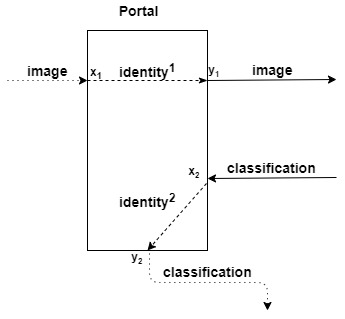
\includegraphics[width=6cm,height=5cm]{portal1.jpg}
\centering
\caption{Portal.
\label{portal1}}

\end{figure}


 The Figure~\ref{portal1} is also an informal representation of the formal syntax of Governed Components and Typing language that we are going to introduce in the following sections.  
 
 The component has an interface denoted by $\interface{x_1,x_2}{y_1,y_2}$ (introduced in~\ref{Syntax of Governed Components}) where $x_1,x_2$ are the \textit{input ports} and $y_1,y_2$ are the \textit{output ports}. On the input ports the component can always receive values. Since we have reactive components, in the sence that are triggered by an external stimulus, component $K_{portal}$ is able to output as soon as all the values needed (for computing an output value) are received. With dashed arrows ($\dashrightarrow$) we represent the \textit{Local binders} that are the functions, or the way of computing the values for the output. For example: $\xdashrightarrow{\text{$identity^1$}}$ is the local binder represented as an $identity$ function. We put the specific functions for better understanding of the scenario in the examples, but in this work the local binders will be an abstract functions, hence we do not specify them.
 

Capturing the behaviour of a component by looking it as a blackbox, the type should obtain the two main information: First, declared input ports together with a type of values that component should receives on them. Second, the conditions that each output port should meet in order to be able to output a value. In this way, we do not just capture which are the output ports, but we also attach to each of them something we call \textit{constraints}. This attachment serves for the purpose of declaring the following: the type of value that can be output from the specific port, the maximum number of values that the port is able to send, and the most important the \textit{dependency}. The \textit{dependency} announces on which input ports does component need to receive a value in order for the input to be computed.  

The \textit{type} of component $K_{portal}$ describes the following (Section~\ref{Syntax of Typing language}): The component has two input ports $x_1$ and $x_2$ where on one can always receive images and on the other one $class$ denoted by $\depen{x_1}{image},\depen{x_2}{class}$. The constraints for the port $y_1$ are the following: Port $y_1$ can output a value of the type $image$ as soon as some value is received on port $x_1$ denoted by $\constr{y_1}{image}{\infty}{\pev{x_1}{N}}$. The infinity claims that $y_1$ can output unbounded number of $images$, while $N$ is the number of values that $y_1$ received from $x_1$ that are still waiting to be precessed. Similar to abstracting the functions for the local binders, we also abstract the type of a values that are received/sent, but still for the sake of understanding the examples we put the specific types ($image$, $class$, $ID$...). As you can notice, the type does not describe the internal connections directly (in this case local binders) since we are trying to capture the behaviour of the components looking at then as encapsulated entities. 

Next, we have component $K_{storage}$ that is receiving, storing and sending an $image$ and a $class$ and one of its possible graphical representations is shown in Figure~\ref{storage1}. We use this component to illustrate different usages of the local binders. 

\begin{figure}[H]

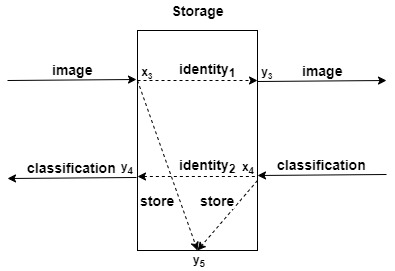
\includegraphics[width=7cm,height=4.5cm]{storage1.jpg}
\centering
\caption{Storage.
\label{storage1}}

\end{figure}


The interface of $K_storage$ consists of two input ports and three output ports ($\interface{x_3,x_4}{y_3,y_4,y_5}$). Let us look at the port $x_3$. The $image$ received on it is used for computing a value that is sent from port $y_3$, but also to be stored on the port $y_5$. The $image$ is equally and at the same time used for both computations. In the same way the value $class$ received on $x_4$ is used in two local binders: it is used to compute a value (in this case, forwarding a value, since it is just an identity function-$identity_2$) for the port $y_4$, but also to be stored on $y_5$. Moreover, if we take a look at the local binder $store$, it needs two values for its computation ($store(image,class)$), which means that its computation \textit{depends} on two values. For example, let the function $store$ be the function that creates a list of pairs $(image,classification)$.  
The $type$ of the component $K_{storage}$ announces the following: The component has two input ports with the specific type of values received on them: $\depen{x_3}{image}, \depen{x_4}{class}$. On its interface has also three output ports: $y_3,y_4$ and $y_5$. Port $y_3$ can output unbounded number of values for the message $image$, but it outputs as soon as a value is received on port $x_3$ ($\constr{y_3}{image}{\infty}{\pev{x_3}{N_1}}$). The similar reasoning for the port $y_4$ ($\constr{y_4}{class}{\infty}{\pev{x_4}{N_2}}$). Instead, the port $y_5$, as already mentioned has two dependencies. The value for that port is computed only if both values ($image$ and $class$) are received: $\constr{y_5}{(image,class)}{\infty}{\pev{x_3}{N_3},\pev{x_4}{N_4}}$. Note that $N$ might be different for the different output ports, even if they depend on the same input port (e.g. $\pev{x_3}{N_1}$ and $\pev{x_3}{N_3}$) because it is not the number of values received on that port during the time, but the number of values received but not used yet.

The description of component $K_{RE}$  and its type we can determine in the same manner as the previous components, where we graphically represent it in the Figure~\ref{re1}.
It has only on input port $x_5$ and one output port $y_2$. The local binder $classify$ is used to compute a value for $y_6$ ($classify(x_5)$).

The $type$ says $K_{RE}$ has the input port $x_5$ on which can receive the values of the type $image$. The only constraint is $\constr{y_6}{class}{\infty}{\pev{x_5}{N}}$, that describes the conditions to output the value from $y_6$. 

\begin{figure}[H]

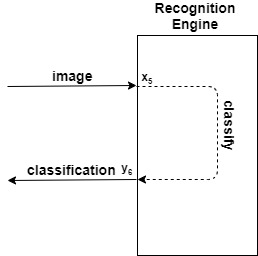
\includegraphics[width=4.2cm,height=4cm]{re1.jpg}
\centering
\caption{Recognition Engine.
\label{re1}}

\end{figure}

The three components described above are called $base\  components$. They cannot be decomposed since they are the special units used to build the composite component, but they are not composite itself. What is specific for a base components is that they are the only ones that have local binders, and as for a type, the number of values that output ports are capable to output is always unbounded (as long as it is not put in an environment where this boundary can be changed).

Since we already mentioned the IRC protocol were the $roles$ \portal, \storage $ $ and \re $ $ participate in, let us now gather the $base\ components$ described above together with some protocol to build a $composite component$.  

The expected interaction among these roles can be described as IRC protocol (\girc), choreographically written as follows:
\begin{flushleft}
    

\begin{tabular}{l l l l}
 
\girc $=$ & \portal & $\xrightarrow{\text{image}}$ & \storage;\\

& \storage & $\xrightarrow{\text{image}}$ & \re;\\

&  \re & $\xrightarrow{\text{classification}}$ & \storage; \\

&  \storage & $\xrightarrow{\text{classification}}$ & \portal\\

\end{tabular}
\end{flushleft}

This is the intuitive representation of the protocol where its syntax we show in the following section. Let the prescribed communication from the above be repeated over and over again (recursion).

The protocol declares the following: \portal $ $ sends an $image$ to \storage $ $ for the $image$ to be saved, after which, \storage $ $ immediately reacts by sending that image to \re $ $ to be processed-classified. After that, \re $ $ sends the determined $class$ to the storage to be saved together with the original image and \storage $ $ communicates with \portal $ $ by sending the image $class$ to it. 

To implement a system ruled by IRC protocol, we may use \textit{off-the-shelf} modules implementing different roles, ensuring that they behave according to the protocol. For example, \portal $ $ could
be implemented by the following component $K_{portal}$, \storage $ $ by $K_{storage}$ and \re $ $ by $K_{RE}$.







In the Figure~\ref{irc1} we have the Image Recognition Component. It contains three $subcomponents$: $K_{portal}$, $K_{storage}$ and $K_{RE}$ together with IRC protocol ($G_{IRC}$). Moreover it contains connections (connection binders) between subcomponents for the purpose of message exchange (full line arrows). For example, the binder $\dbinder{\lab}{\mathbf{Portal}}{y_1}{\roleport{\mathbf{Storage}}{x_3}}$ ensures that the message ``image'' from port $y_1$ of role \portal $ $ is sent to  role \storage $ $ on port $x_3$. We also have forwarders that forward the message to/from an external environment. The $composite\ component$ is a component itself, and can be used in different contexts (for the purpose of reuse).
Only one subcomponent can have the special $role$ of receiving the values from and sending the values to the external environment (in this example it is $K_{portal}$). 


\begin{figure}[H]

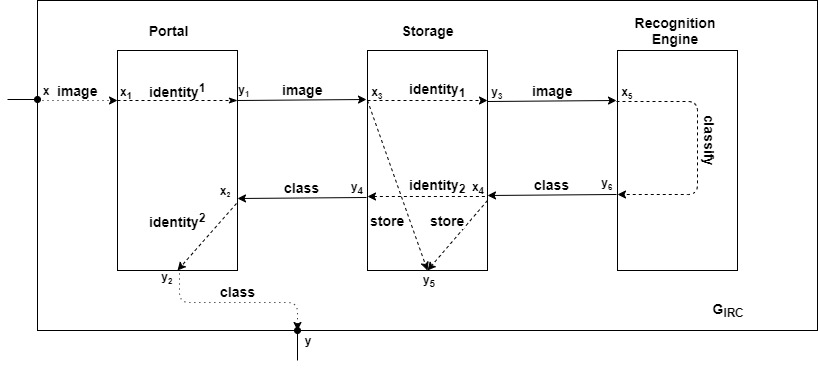
\includegraphics[width=\textwidth, height=7cm]{graph1.jpg}
\centering
\caption{Image Recognition Component.
\label{irc1}}

\end{figure}


The $type$ of IRC component, that is the composite component, describes the component's behaviour in the same way as it does for the base components. However, capturing it requires some methods to establish the connection between the interface of IRC component and the internal scenario, since the $type$ describes the abilities of the interface (input/output ports). 
Moreover, since the component $K_{portal}$ is the only component that has the communication with an external interface, the main focus when describing a type of the composite component will be on it. 
Lets assume that all the subcomponents (internal ones) are well-typed, and that they can carry-out the protocol $G_{IRC}$. Focusing on the ports $x$ and $y$ from the interface we have the following conclusion: The $type$ declares: IRC has one input port $x$ on which receives the values of the type $image$. The challenging part is to determine the constraints for the output port. Looking at $y$ we can notice that its value is the one directly forwarded from the port $y_2$, hence, all the constraints that we have for $y_2$ are the same for the output port $y$. Values for computing the output for $y_2 $ (which means also for $y$) depend on the values received on the port $x_2$. This kind of dependency are denoted as $direct$ dependencies. The problem is that at the end, we do not want to see any dependencies on the internal ports (ports on the interface of the subcomponents), but we want to capture if there is a dependency on $x$. The process of concluding the right constraints is ''backwards`` (so, if there is a dependency on $x$ we call it \textit{transitive} dependency). So, $x_2$ will have an input received from a message $class$ given by the protocol. Since we are focusing only on $K_{portal}$ we can notice that due to the protocol, before  it receives the message $class$, $K_{portal}$ needs to output the value from the port $y_1$. As already seen in the previous examples, $y_1$ needs a value to be received on $x_1$ each time it wants to output. Since the values that $x_1$ receives are directly forwarded from the port $x$ we can conclude that port $y$ needs a value to be received on port $x$ each time it wants to output. Since we said that the protocol is repeated over and over again (recursive protocol), and since all the output ports can send a value unbounded time, the constraint for $y$ is the following: $\constr{y}{class}{\infty}{\pev{x}{N}}$. 

If, for example, we take the protocol $G_{IRC}$ as ``one shot'' protocol (non recursive protocol that, after communication is done once, terminates), that would change the boundary in the constraint, since there would be only one value sent for $y$ to be computed, since the protocol after sending one value on $x_2$ will end (``one shot'' protocol that terminates). But not only that, since we are ``losing'' the dependency on $x$ after first value received, the dependency in not denoted as \textit{per each value} dependency anymore. The new kind of dependency that we have now is called ``initial dependency''. In that case the constraint would be: $\constr{y}{class}{1}{\ind{x}}$. 

In the examples above each output port was dependent on some input port. We have seen how it can be dependent on one or more inputs, but also that more than one port can depend on the value coming from the same recipient. However, these are not the only cases. We can have a port that gives us a value every time needed, without dependency. In Figure~\ref{irc2} it is graphically represented another \textit{Image recognition component}. The subcomponent  $K_{portal}$ every time some prescribed protocol requires an output on the ports $y_2$ and $y_3$, the component $K_{portal}$ is able to provide it. In this example, $K_{portal}$ knows the current date and gives a random unique ID (even if image was not uploaded since the data is collected due FIFO method).



\begin{figure}[H]

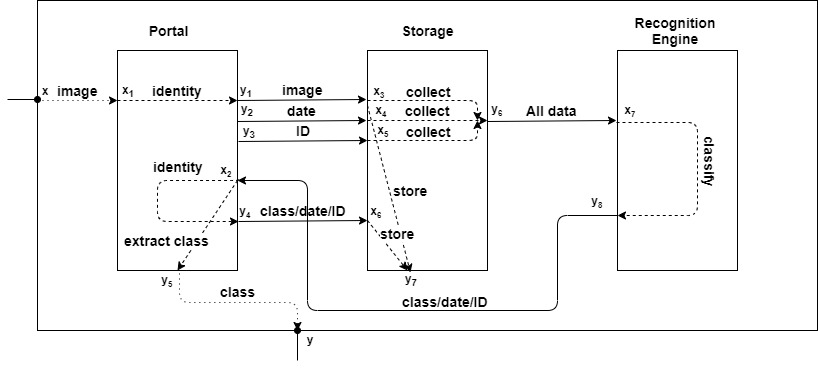
\includegraphics[width=\textwidth, height=7cm]{graph2.jpg}
\centering
\caption{Image recognition component.
\label{irc2}}

\end{figure}




Gathering components together with a protocol we might obtain the closed system, that is a component itself (Figure~\ref{user}). From the point of view of Governed Components language it makes sense to describe this component like in the examples above. On the other hand, since it has an empty interface and cannot make a further communication with other components, which interferes with reusability, it will have an ``empty'' type.


\begin{figure}[H]

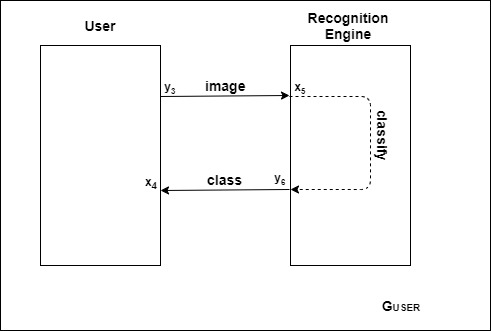
\includegraphics[width=7cm, height=4cm]{user.jpg}
\centering

\caption{Composite component with an empty interface.
\label{user}}
\end{figure}




